\chapter{Fonctions d’onde, matrices densité et localité}

\lectureoverview{Le théorème de Bell est reporté pour une raison essentielle : avant de demander ce que Bell interdit, il faut définir précisément l’intrication. Un état bipartite est intriqué s’il ne peut pas se factoriser en un état pour Alice et un état pour Bob. Les fonctions d’onde rendent ce critère concret, les corrélations en révèlent les conséquences et l’état singulet en fournit l’exemple décisif. La matrice densité réduite devient alors la description locale complète d’une partie d’un tout intriqué. Une fois ces outils en place, la mesure apparaît comme une interaction qui produit de l’intrication, la frontière système--observateur peut être déplacée sans modifier les prédictions, et la tension apparente entre intrication et localité peut être formulée avec précision : les choix effectués à distance modifient les corrélations conditionnelles, mais pas les statistiques non conditionnelles disponibles pour transmettre un signal.}

\section{Ce que signifie réellement l’intrication}

Il est tentant de passer directement au théorème de Bell. Ce théorème est remarquable, mais sa portée ne peut être dissociée de la structure qu’il met à l’épreuve. La question la plus pressante n’est donc pas encore de savoir si la mécanique quantique viole une inégalité de Bell, mais ce qu’un état intriqué nous apprend sur un système composé.

On dit souvent que deux systèmes intriqués \emph{partagent un état}. Cette expression ne permet de rien distinguer. Tout système composé possède un état, qu’il soit intriqué ou non. La distinction tient à la factorisation. Si \(A\) et \(B\) ont pour espaces de Hilbert \(\mathcal H_A\) et \(\mathcal H_B\), l’état de la paire appartient à
\begin{equation}
\mathcal H_{AB}=\mathcal H_A\otimes\mathcal H_B.
\end{equation}
Un état pur est un état produit lorsqu’il peut s’écrire
\begin{equation}
\ket{\Psi}_{AB}=\ket{\psi}_A\otimes\ket{\phi}_B.
\label{eq:l7-product-state}
\end{equation}
Si aucune paire de facteurs de ce type n’existe, \(\ket{\Psi}_{AB}\) est intriqué.

\begin{classroomqa}
\audiencequestion{L’intrication signifie-t-elle simplement que les deux systèmes figurent dans un même vecteur d’état ?}
\lecturerresponse{Non. Un état produit appartient lui aussi à l’espace de Hilbert de la paire entière. L’intrication est une affirmation plus forte, indépendante de la base : le vecteur du système entier ne peut pas s’écrire comme le produit tensoriel d’un vecteur pour Alice et d’un vecteur pour Bob.}
\end{classroomqa}

\begin{classroomqa}
\audiencequestion{Un changement de base astucieux pourrait-il transformer un état intriqué en état produit ?}
\lecturerresponse{Pas si le changement de base est local, c’est-à-dire s’il consiste en un changement de base pour Alice et un autre pour Bob. Les changements de base locaux modifient les coordonnées de chaque facteur, mais pas la factorisation de l’état. Une base quelconque de l’espace de Hilbert conjoint peut masquer la structure de produit tensoriel, mais elle ne change pas les degrés de liberté physiques qui appartiennent à Alice et à Bob.}
\end{classroomqa}

\section{Les fonctions d’onde comme coordonnées dans l’espace de Hilbert}

Le terme \emph{fonction d’onde}évoque une image historique qui ne fait pas partie de sa définition mathématique. Une fonction d’onde est la représentation par coordonnées d’un vecteur d’état dans une base choisie. Soit un ensemble complet d’observables commutables, doté de vecteurs propres simultanés
\begin{equation}
\ket{a,b,c,\ldots}.
\end{equation}
Les indices doivent être complets : pris ensemble, ils distinguent chaque vecteur de la base. Alors
\begin{align}
\ket{\Psi}
&=\sum_{a,b,c,\ldots}
\ket{a,b,c,\ldots}
\braket{a,b,c,\ldots}{\Psi} \\
&=\sum_{a,b,c,\ldots}
\psi(a,b,c,\ldots)\ket{a,b,c,\ldots},
\label{eq:l7-wavefunction-expansion}
\end{align}
où
\begin{equation}
\psi(a,b,c,\ldots)
=\braket{a,b,c,\ldots}{\Psi}.
\label{eq:l7-wavefunction-definition}
\end{equation}
Pour des indices continus, les sommes correspondantes deviennent des intégrales.

\begin{figure}[htbp]
\centering
\includegraphics[width=0.88\textwidth]{lecture_07_figure_01.png}
\caption{La fonction d’onde comme ensemble des coefficients d’un état dans une base complète.}
\lectureframe{00:07:00}
\end{figure}

Pour une particule dans l’espace tridimensionnel, les indices de commutation peuvent être \(x,y,z\), et
\begin{equation}
\psi(x,y,z)=\braket{x,y,z}{\Psi}
\end{equation}est la fonction d’onde usuelle de Schr\"odingeren représentation de position. Pour un spin dans la base \(\sigma_z\), la fonction d’onde se réduit à la paire
\begin{equation}
\psi(u)=\braket{u}{\Psi},
\qquad
\psi(d)=\braket{d}{\Psi}.
\end{equation}
Pour deux spins, il faut deux indices :
\begin{equation}
\Psi(a,b)=\braket{a,b}{\Psi},
\qquad
a,b\in\{u,d\}.
\label{eq:l7-two-spin-wavefunction}
\end{equation}
Cette définition n’exige nullement l’existence d’une onde littérale dans l’espace.

\begin{classroomqa}
\audiencequestion{Un changement de base de la fonction d’onde est-il une transformée de Fourier ?}
\lecturerresponse{La transformée de Fourier est le changement de base particulier qui relie les représentations en position et en impulsion. Plus généralement, tout changement de base orthonormée est une transformation unitaire des coordonnées. Le passage de la base \(\sigma_z\)à la base \(\sigma_x\)est analogue à une transformée de Fourier, même s’il s’agit d’une matrice unitaire de dimension finie plutôt que d’une transformée intégrale position--impulsion.}
\end{classroomqa}

\begin{classroomqa}
\audiencequestion{Si la fonction d’onde change lors d’un changement de base, l’état physique a-t-il changé ?}
\lecturerresponse{Non. Le ket \(\ket{\Psi}\)est l’état abstrait. Les nombres \(\psi(a,b,c,\ldots)\)sont ses coordonnées dans une base choisie. Le changement de coordonnées modifie ces nombres, mais laisse inchangés le vecteur et toutes les prédictions physiques.}
\end{classroomqa}

\section{Valeurs moyennes en composantes}

Avant d’introduire les matrices densité, explicitons la structure en composantes d’une valeur moyenne. Soit \(L\)une observable, dont les éléments de matrice sont
\begin{equation}
L_{a'a}=\bra{a'}L\ket{a}.
\label{eq:l7-matrix-elements}
\end{equation}
Si \(\ket{\Psi}=\sum_a\psi(a)\ket{a}\), alors
\begin{align}
\expect{L}
&=\bra{\Psi}L\ket{\Psi} \\
&=\sum_{a',a}
\psi^*(a')\bra{a'}L\ket{a}\psi(a) \\
&=\sum_{a',a}\psi^*(a')L_{a'a}\psi(a).
\label{eq:l7-expectation-components}
\end{align}

\begin{figure}[htbp]
\centering
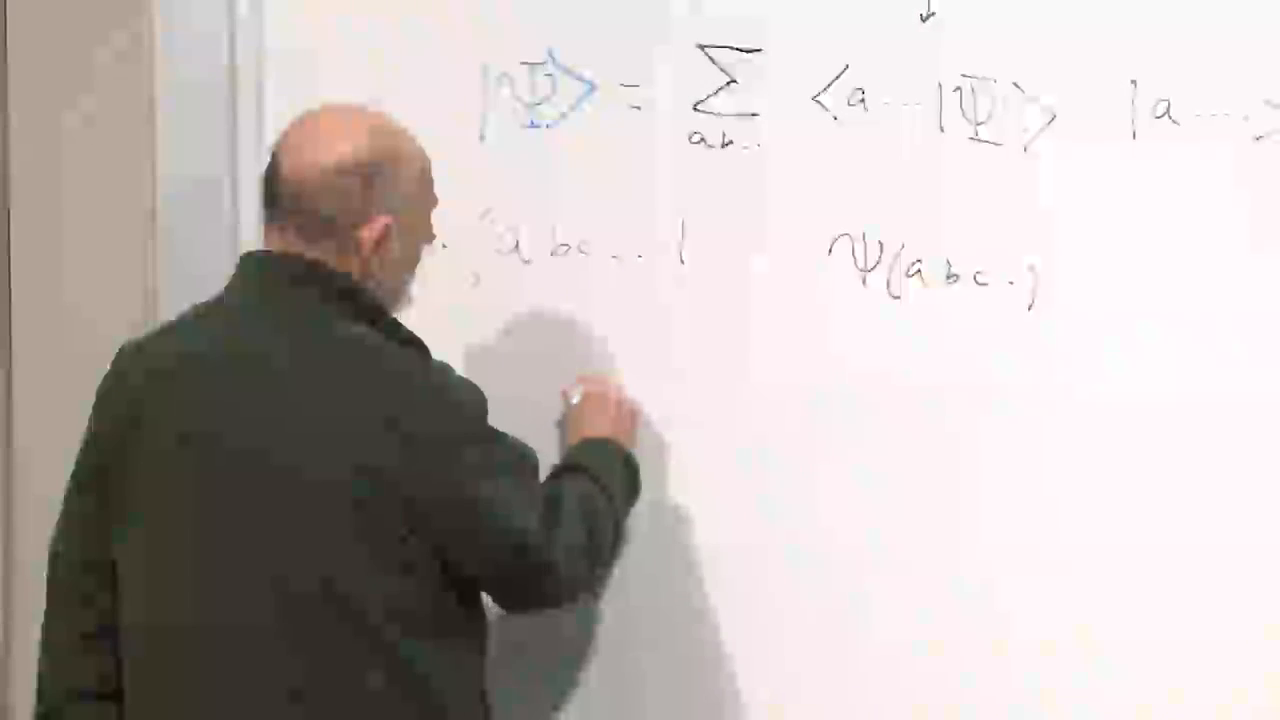
\includegraphics[width=0.88\textwidth]{lecture_07_figure_02.png}
\caption{Développement de la valeur moyenne en sandwich à l’aide des coefficients de la fonction d’onde et des éléments de matrice.}
\lectureframe{00:14:08}
\end{figure}

Divisons maintenant le système en une partie appartenant à Alice et une autre à Bob. Soit \(a\)un indice de base complet pour Alice et \(b\)un indice de base pour Bob :
\begin{equation}
\ket{\Psi}_{AB}
=\sum_{a,b}\Psi(a,b)\ket{a,b}.
\label{eq:l7-composite-expansion}
\end{equation}
Une observable appartenant uniquement à Alice est représentée dans l’espace composé par
\begin{equation}
L_A=L\otimes I_B,
\end{equation}
Ses éléments de matrice sont donc
\begin{equation}
\bra{a',b'}L_A\ket{a,b}
=L_{a'a}\delta_{b'b}.
\label{eq:l7-alice-local-matrix}
\end{equation}
De même, une observable locale à Bob s’écrit
\begin{equation}
M_B=I_A\otimes M,
\qquad
\bra{a',b'}M_B\ket{a,b}
=\delta_{a'a}M_{b'b}.
\label{eq:l7-bob-local-matrix}
\end{equation}
L’identité dans le facteur qui n’est pas concerné exprime mathématiquement que l’opération d’Alice agit sur Alice et celle de Bob sur Bob.

En substituant l’équation~\eqref{eq:l7-alice-local-matrix}dans l’expression de la valeur moyenne, on obtient
\begin{equation}
\expect{L_A}
=\sum_{a',a,b}
\Psi^*(a',b)L_{a'a}\Psi(a,b).
\label{eq:l7-local-expectation}
\end{equation}
Cette formule contient déjà la matrice densité réduite ; nous la réorganiserons après avoir examiné ce qu’implique la factorisation.

\begin{classroomqa}
\audiencequestion{Pourquoi ne reste-t-il qu’un seul indice de Bob dans l’équation~\eqref{eq:l7-local-expectation}?}
\lecturerresponse{L’identité dans l’espace de Bob contribue un facteur \(\delta_{b'b}\). Elle impose l’égalité des indices du bra et du ket du côté de Bob ; la double somme sur \(b',b\)se réduit donc à une seule somme sur \(b\).}
\end{classroomqa}

\begin{classroomqa}
\audiencequestion{Alice a-t-elle besoin de savoir quelle base Bob utilise ?}
\lecturerresponse{Aucune prédiction physique ne dépend de la base de Bob. La somme sur une base complète de Bob constitue une résolution de l’identité. Une autre base pour Bob modifie les composantes individuelles \(\Psi(a,b)\), mais pas la valeur moyenne d’Alice.}
\end{classroomqa}

\section{États produits et corrélations}

Dans un état produit, la fonction d’onde conjointe se factorise :
\begin{equation}
\Psi(a,b)=\psi_A(a)\phi_B(b).
\label{eq:l7-wavefunction-factorization}
\end{equation}
Substituons cela dans l’équation~\eqref{eq:l7-local-expectation}:
\begin{align}
\expect{L_A}
&=\sum_{a',a,b}
\psi_A^*(a')\phi_B^*(b)
L_{a'a}
\psi_A(a)\phi_B(b) \\
&=\left[
\sum_{a',a}\psi_A^*(a')L_{a'a}\psi_A(a)
\right]
\left[
\sum_b|\phi_B(b)|^2
\right] \\
&=\bra{\psi_A}L\ket{\psi_A}.
\label{eq:l7-product-local-expectation}
\end{align}
La normalisation de Bob rend son facteur égal à un. Alice a donc exactement les mêmes statistiques locales que si le système de Bob n’avait jamais été introduit.

\begin{figure}[htbp]
\centering
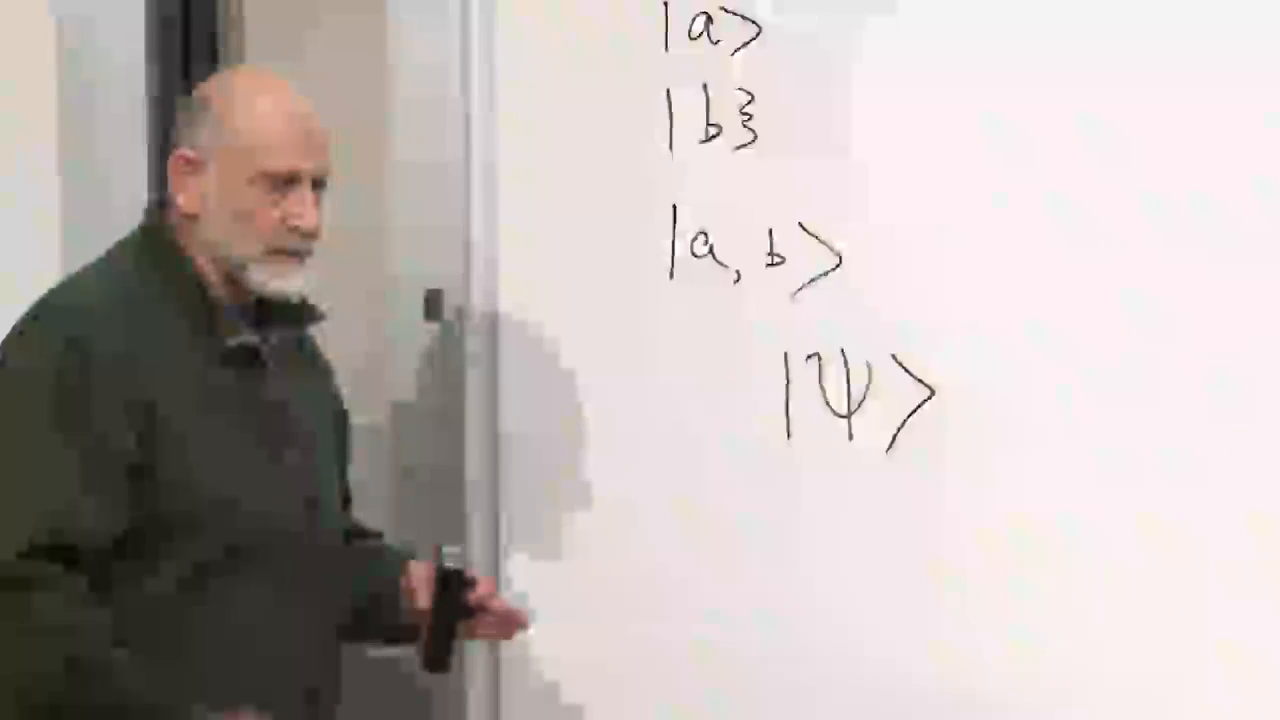
\includegraphics[width=0.88\textwidth]{lecture_07_figure_03.png}
\caption{Factorisation de la fonction d’onde conjointe et séparation correspondante des valeurs moyennes locales.}
\lectureframe{00:29:18}
\end{figure}

Le produit d’une observable d’Alice par une observable de Bob a pour éléments de matrice
\begin{equation}
\bra{a',b'}L_A M_B\ket{a,b}
=L_{a'a}M_{b'b}.
\end{equation}
Dans un état produit, sa valeur moyenne se factorise :
\begin{equation}
\expect{L_A M_B}
=\expect{L_A}\expect{M_B}.
\label{eq:l7-product-correlation-factorization}
\end{equation}
Il est donc naturel de définir la corrélation connectée
\begin{equation}
C(L,M)
=\expect{L_A M_B}
-\expect{L_A}\expect{M_B}.
\label{eq:l7-connected-correlation}
\end{equation}
Pour tout état produit et toute paire d’observables locales, \(C(L,M)=0\). Réciproquement, pour un état bipartite pur intriqué, il existe une paire d’observables locales dont la corrélation connectée est non nulle.

\begin{classroomqa}
\audiencequestion{\(L_A M_B\)signifie-t-il que Bob est mesuré d’abord, puis Alice ?}
\lecturerresponse{Non. Les opérateurs agissent sur les vecteurs d’état ; ce sont les appareils qui effectuent les mesures. Le produit signifie que \(M_B\)agit, puis que \(L_A\)agit. Comme les opérateurs agissent dans des facteurs tensoriels différents, \([L_A,M_B]=0\), et leur ordre mathématique est donc sans importance. Le protocole expérimental servant à estimer la valeur moyenne conjointe est une question distincte.}
\end{classroomqa}

\begin{classroomqa}
\audiencequestion{L’état peut-il être intriqué même si une corrélation particulière s’annule ?}
\lecturerresponse{Bien sûr. Si \(C(L,M)\)s’annule, cela signifie seulement que cette paire particulière d’observables n’est pas corrélée. Pour établir la factorisation d’un état pur, toutes les corrélations croisées locales doivent se factoriser. Une corrélation partielle ne correspond pas nécessairement non plus à une intrication partielle mesurable par un simple nombre ; le spectre complet de la matrice densité réduite contient cette information.}
\end{classroomqa}

\begin{classroomqa}
\audiencequestion{Tout état corrélé est-il intriqué ?}
\lecturerresponse{Pour les états purs considérés ici, des corrélations qui ne se factorisent pas révèlent l’intrication. Pour les états mixtes, des corrélations classiques ordinaires peuvent aussi rendre \(C(L,M)\neq0\). Le critère fondé sur la matrice densité, que nous verrons plus loin, doit donc être assorti d’une précision : il faut savoir si l’état du système entier est pur.}
\end{classroomqa}

\section{Le singulet : un tout défini aux parties indéterminées}

Soit \(\boldsymbol{\sigma}\)l’opérateur agissant sur le spin de Bob et \(\boldsymbol{\tau}\)celui agissant sur le spin d’Alice. Leur état singulet est
\begin{equation}
\ket{S}
=\frac{1}{\sqrt2}
\left(\ket{u d}-\ket{d u}\right),
\label{eq:l7-singlet}
\end{equation}
où le premier emplacement correspond à Bob et le second à Alice. Aucun des deux spins n’a de composante \(z\)bien définie :
\begin{equation}
\expect{\sigma_z}=0,
\qquad
\expect{\tau_z}=0.
\label{eq:l7-singlet-local-z}
\end{equation}
Pourtant, leur produit est certain :
\begin{equation}
\expect{\sigma_z\tau_z}=-1.
\label{eq:l7-singlet-product-z}
\end{equation}
Toute mesure selon \(z\)donne des résultats opposés.

L’invariance par rotation rend cette affirmation indépendante de la direction. Pour tout vecteur unitaire \(\mathbf n\),
\begin{equation}
\expect{\boldsymbol{\sigma}\cdot\mathbf n}
=\expect{\boldsymbol{\tau}\cdot\mathbf n}=0,
\qquad
\expect{
(\boldsymbol{\sigma}\cdot\mathbf n)
(\boldsymbol{\tau}\cdot\mathbf n)
}=-1.
\label{eq:l7-singlet-any-axis}
\end{equation}
Plus généralement,
\begin{equation}
\expect{\sigma_i\tau_j}=-\delta_{ij}.
\label{eq:l7-singlet-correlation-tensor}
\end{equation}
Chaque partie est complètement non polarisée, tandis que les résultats obtenus selon un même axe sont parfaitement anticorrélés.

\begin{figure}[htbp]
\centering
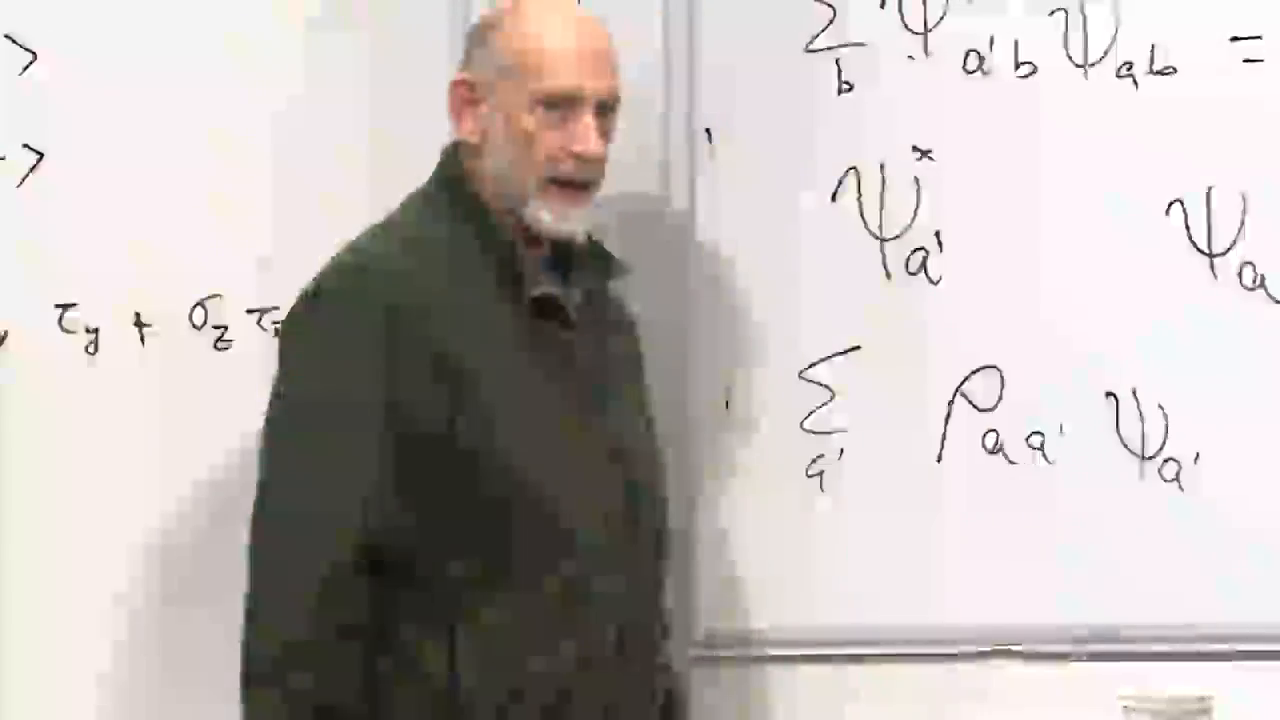
\includegraphics[width=0.88\textwidth]{lecture_07_figure_04.png}
\caption{Pour le singulet, la valeur moyenne de chaque spin local s’annule, tandis que le produit des composantes selon un même axe vaut \(-1\).}
\lectureframe{00:38:28}
\end{figure}

C’est l’inversion caractéristique produite par l’intrication. Pour un spin isolé dans un état pur, il existe une direction selon laquelle son spin est bien défini. Dans le singulet, aucune direction ne rend bien défini le spin local de l’un ou l’autre des systèmes. Pourtant, l’état composé est pur et entièrement spécifié. Nous connaissons le tout aussi complètement que le permet la mécanique quantique, sans pouvoir assigner un état pur à l’une ou l’autre de ses parties.

\begin{classroomqa}
\audiencequestion{Si l’état du tout est connu exactement, pourquoi ne pouvons-nous pas en déduire un état bien défini pour chaque spin ?}
\lecturerresponse{Parce que le singulet n’est pas un état produit. Ses coefficients ne se décomposent pas en une amplitude de Bob multipliée par une amplitude d’Alice. L’information réside dans les relations entre les parties plutôt que dans deux fonctions d’onde locales existant indépendamment.}
\end{classroomqa}

\begin{classroomqa}
\audiencequestion{Un opérateur tel que \(\sigma_z\)peut-il lui-même être un état possible du spin ?}
\lecturerresponse{Non. Un état est un vecteur ou, plus généralement, un opérateur densité ; \(\sigma_z\)est une observable qui agit sur les états. Un vecteur propre de \(\sigma_z\)est un état dans lequel la composante \(z\)est bien définie, mais l’observable et ses vecteurs propres sont des objets de nature différente.}
\end{classroomqa}

\begin{classroomqa}
\audiencequestion{Quand nous écrivons \(\sigma_z\tau_z\ket{S}=-\ket{S}\), avons-nous effectué une mesure ?}
\lecturerresponse{Non. L’équation décrit l’action d’un opérateur sur un vecteur. Elle indique qu’une mesure de l’observable conjointe correspondante donnerait certainement \(-1\), mais écrire l’équation aux valeurs propres n’introduit aucun détecteur.}
\end{classroomqa}

\begin{classroomqa}
\audiencequestion{Une paire intriquée peut-elle n’être que partiellement corrélée ?}
\lecturerresponse{Oui. L’anticorrélation parfaite est une propriété particulière du singulet pour des axes identiques. D’autres états intriqués peuvent présenter des corrélations plus faibles, et même le singulet donne \(-\mathbf a\cdot\mathbf b\)plutôt que \(-1\)lorsque les deux axes diffèrent. L’intrication concerne la non-factorisation, et non l’accord ou le désaccord parfait pour chaque mesure choisie.}
\end{classroomqa}

\section{Préparer le singulet par relaxation énergétique}

L’opérateur à deux spins invariant par rotation
\begin{equation}
\boldsymbol{\sigma}\cdot\boldsymbol{\tau}
=\sigma_x\tau_x+\sigma_y\tau_y+\sigma_z\tau_z
\label{eq:l7-spin-dot-spin}
\end{equation}
organise l’espace d’états de dimension quatre. Sur le singulet,
\begin{equation}
(\boldsymbol{\sigma}\cdot\boldsymbol{\tau})\ket{S}
=-3\ket{S},
\label{eq:l7-singlet-dot-eigenvalue}
\end{equation}
tandis que chacun des trois états triplets a pour valeur propre \(+1\).

\begin{figure}[htbp]
\centering
\includegraphics[width=0.88\textwidth]{lecture_07_figure_05.png}
\caption{Le couplage invariant par rotation \(\boldsymbol{\sigma}\cdot\boldsymbol{\tau}\)et son rôle dans la séparation des secteurs singulet et triplet.}
\lectureframe{00:52:33}
\end{figure}

Supposons que l’hamiltonien d’interaction contienne
\begin{equation}
H_{\mathrm{int}}
=J\,\boldsymbol{\sigma}\cdot\boldsymbol{\tau}.
\label{eq:l7-exchange-hamiltonian}
\end{equation}
Pour un couplage antiferromagnétique \(J>0\), le singulet se situe en dessous du triplet de
\begin{equation}
\Delta E=4J.
\end{equation}
Rapprochons les spins, laissons les composantes d’énergie supérieure se désexciter en émettant un photon, un phonon ou une autre excitation ; la paire se relaxe alors vers le singulet. On peut ensuite éloigner les spins tout en préservant leur état conjoint, à condition que leur séparation n’entraîne pas de rotations de spin incontrôlées et que l’écart énergétique ne se ferme pas trop brusquement.

La même logique énergétique apparaît dans les systèmes atomiques. Dans le positronium, par exemple, le couplage des spins de l’électron et du positron sépare les configurations singulet et triplet. Une différence d’énergie correspond aussi à une différence de masse par \(E=mc^2\), bien que la spectroscopie exprime généralement le dédoublement en énergie ou en fréquence.

\begin{classroomqa}
\audiencequestion{Le singulet est-il toujours l’état fondamental de deux spins en interaction ?}
\lecturerresponse{Non. C’est l’état fondamental pour le signe \(J>0\)dans l’équation~\eqref{eq:l7-exchange-hamiltonian}. Le signe opposé place le triplet plus bas en énergie. L’argument de préparation dépend de l’interaction réelle et de l’ordre énergétique des états, et pas simplement de la présence de deux spins.}
\end{classroomqa}

\begin{classroomqa}
\audiencequestion{Peut-on mesurer \(\boldsymbol{\sigma}\cdot\boldsymbol{\tau}\)en mesurant séparément les trois composantes ?}
\lecturerresponse{Pas sur une seule paire au moyen de trois mesures simultanées du spin local : \(\sigma_x,\sigma_y,\sigma_z\)sont incompatibles, tout comme les trois composantes de \(\tau\). On peut reconstituer sa valeur moyenne à partir de trois sous-ensembles mesurés selon \(x,y,z\), ou mesurer directement l’observable singulet--triplet à l’aide d’un appareil conjoint adapté.}
\end{classroomqa}

\begin{classroomqa}
\audiencequestion{Après la séparation des spins, doivent-ils continuer à interagir pour rester intriqués ?}
\lecturerresponse{Non. Une interaction est nécessaire pour préparer ou modifier l’état, mais une fois le singulet préparé, l’évolution unitaire peut préserver son intrication sans force persistante entre les particules. Des champs magnétiques locaux peuvent faire tourner les deux facteurs, mais les rotations unitaires locales ne détruisent pas à elles seules l’intrication.}
\end{classroomqa}

\section{La matrice densité réduite}

Revenons à la valeur moyenne locale d’Alice :
\begin{equation}
\expect{L_A}
=\sum_{a',a,b}
\Psi^*(a',b)L_{a'a}\Psi(a,b).
\end{equation}
Regroupons les facteurs qui ne concernent pas \(L\):
\begin{equation}
\expect{L_A}
=\sum_{a',a}
\left[
\sum_b\Psi(a,b)\Psi^*(a',b)
\right]L_{a'a}.
\label{eq:l7-regrouped-expectation}
\end{equation}
L’expression entre crochets est la matrice densité réduite d’Alice,
\begin{equation}
(\rho_A)_{aa'}
=\sum_b\Psi(a,b)\Psi^*(a',b).
\label{eq:l7-reduced-density-components}
\end{equation}
En notation indépendante de la base,
\begin{equation}
\rho_A
=\operatorname{Tr}_B\ket{\Psi}\bra{\Psi},
\label{eq:l7-partial-trace}
\end{equation}
et toute valeur moyenne d’une observable locale à Alice est donnée par
\begin{equation}
\expect{L_A}
=\operatorname{Tr}_A(\rho_A L).
\label{eq:l7-density-expectation}
\end{equation}

\begin{figure}[htbp]
\centering
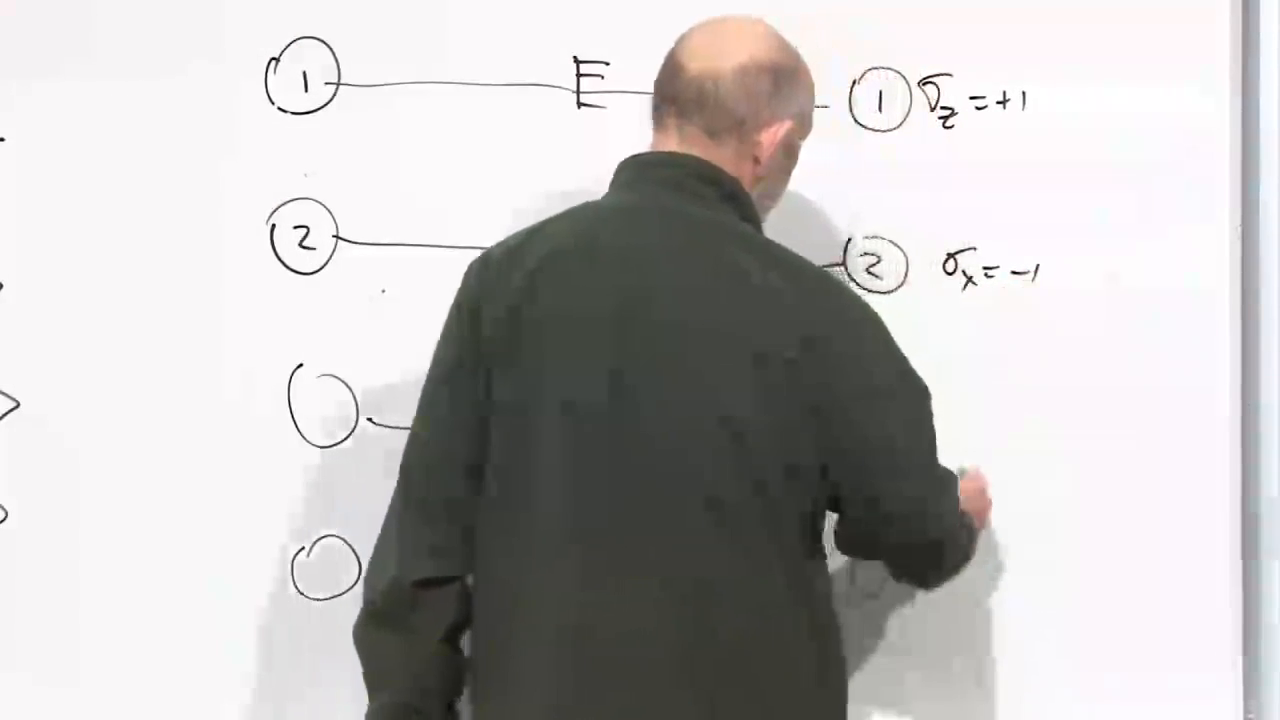
\includegraphics[width=0.88\textwidth]{lecture_07_figure_06.png}
\caption{Matrice densité d’Alice obtenue en sommant les amplitudes conjointes sur l’indice de base de Bob.}
\lectureframe{01:02:33}
\end{figure}

La matrice densité réduite est hermitienne, positive et normalisée :
\begin{equation}
\rho_A^\dagger=\rho_A,
\qquad
\bra{\chi}\rho_A\ket{\chi}\geq0,
\qquad
\operatorname{Tr}\rho_A=1.
\label{eq:l7-density-properties}
\end{equation}
Elle contient exactement l’information nécessaire à toutes les mesures limitées à Alice. Si deux états globaux produisent la même \(\rho_A\), aucune expérience menée par Alice seule ne peut les distinguer.

\begin{classroomqa}
\audiencequestion{Alice mesure-t-elle la matrice densité comme une observable unique ?}
\lecturerresponse{Pas en une seule mesure. La matrice densité est l’objet à partir duquel on calcule toutes les probabilités de mesure locales. À partir de nombreux systèmes préparés de façon identique, Alice peut la reconstituer par tomographie : elle mesure un ensemble suffisant d’observables et déduit la matrice de leurs valeurs moyennes.}
\end{classroomqa}

\begin{classroomqa}
\audiencequestion{Pourquoi sommer sur Bob plutôt que choisir l’un de ses états ?}
\lecturerresponse{Parce qu’Alice ne dispose d’aucune information sur le résultat obtenu par Bob. La trace partielle somme sur une base complète de Bob et donne l’état local non conditionnel. Choisir plutôt un résultat de Bob produirait un état conditionnel ; c’est une opération différente, qui exige de connaître ce résultat.}
\end{classroomqa}

Pour un état produit \(\Psi(a,b)=\psi_A(a)\phi_B(b)\),
\begin{align}
(\rho_A)_{aa'}
&=\sum_b
\psi_A(a)\phi_B(b)
\psi_A^*(a')\phi_B^*(b) \\
&=\psi_A(a)\psi_A^*(a')
\sum_b|\phi_B(b)|^2 \\
&=\psi_A(a)\psi_A^*(a').
\end{align}
On a donc
\begin{equation}
\rho_A=\ket{\psi_A}\bra{\psi_A}.
\label{eq:l7-pure-projector}
\end{equation}
Il s’agit d’un projecteur de rang un. Son action sur \(\ket{\psi_A}\)est
\begin{equation}
\rho_A\ket{\psi_A}
=\ket{\psi_A}\braket{\psi_A}{\psi_A}
=\ket{\psi_A},
\label{eq:l7-density-on-state}
\end{equation}
tandis que, pour tout \(\ket{\chi}\)orthogonal à \(\ket{\psi_A}\),
\begin{equation}
\rho_A\ket{\chi}
=\ket{\psi_A}\braket{\psi_A}{\chi}
=0.
\label{eq:l7-density-on-orthogonal}
\end{equation}

\begin{figure}[htbp]
\centering
\includegraphics[width=0.88\textwidth]{lecture_07_figure_07.png}
\caption{Matrice densité d’un état produit agissant comme un projecteur : valeur propre \(1\)dans la direction de \(\ket{\psi_A}\)et \(0\)sur les vecteurs orthogonaux.}
\lectureframe{01:09:43}
\end{figure}

\section{Spectre de la matrice densité et intrication}

Les valeurs propres de \(\rho_A\)sont positives ou nulles et leur somme vaut un. Pour un état pur du système entier :
\begin{itemize}\item une seule valeur propre non nulle, égale à \(1\), caractérise un état produit ;
\item plusieurs valeurs propres non nulles caractérisent un état intriqué ;
\item des valeurs propres égales sur tout le support local disponible correspondent à une intrication maximale.
\end{itemize}
La décomposition de Schmidt rend cette affirmation particulièrement claire :
\begin{equation}
\begin{aligned}
\ket{\Psi}_{AB}
&=\sum_{r=1}^{R}\sqrt{\lambda_r}
\ket{r}_A\ket{r}_B,\\
\lambda_r&\geq0,
\qquad
\sum_r\lambda_r=1.
\end{aligned}
\label{eq:l7-schmidt}
\end{equation}
pour cette décomposition,
\begin{equation}
\rho_A=\sum_{r=1}^{R}\lambda_r\ket{r}_A\bra{r}.
\label{eq:l7-schmidt-density}
\end{equation}
Le rang de Schmidt \(R\)vaut un pour un état produit et est supérieur à un pour un état pur intriqué.

Pour le singulet,
\begin{equation}
\rho_A
=\operatorname{Tr}_B\ket{S}\bra{S}
=\frac12\ket{u}\bra{u}
+\frac12\ket{d}\bra{d}
=\frac12 I.
\label{eq:l7-singlet-reduced-density}
\end{equation}
Ses valeurs propres sont
\begin{equation}
\operatorname{spec}(\rho_A)
=\left\{\frac12,\frac12\right\}.
\end{equation}
L’état local d’Alice est complètement mélangé, bien que l’état de la paire soit pur.

Le spectre suggère une mesure quantitative. L’entropie de von Neumann
\begin{equation}
S(\rho_A)
=-\operatorname{Tr}(\rho_A\log\rho_A)
=-\sum_r\lambda_r\log\lambda_r
\label{eq:l7-entanglement-entropy}
\end{equation}
s’annule pour un état pur produit et atteint \(\log d_A\)pour un état maximalement intriqué lorsque \(d_A\leq d_B\). On peut remettre à plus tard l’étude détaillée de l’entropie ; le spectre suffit déjà à établir la distinction essentielle.

\begin{classroomqa}
\audiencequestion{Toutes les valeurs propres d’une matrice densité réduite d’un état intriqué doivent-elles être non nulles ?}
\lecturerresponse{Non. Il suffit qu’il y en ait plusieurs de non nulles. Si l’espace d’Alice est de grande dimension, un état intriqué peut occuper un sous-espace de Schmidt de dimension inférieure, laissant d’autres valeurs propres nulles. Une intrication maximale signifie que les valeurs propres sont égales sur tout le plus petit des deux sous-systèmes, et non simplement sur un sous-ensemble quelconque choisi arbitrairement.}
\end{classroomqa}

\begin{classroomqa}
\audiencequestion{Une matrice densité réduite mixte suffit-elle à prouver qu’Alice est intriquée avec Bob ?}
\lecturerresponse{Seulement si l’on sait que l’état global est pur. Un état local mixte peut aussi résulter d’un mélange classique ordinaire dans un état global mixte. Pour un état bipartite pur, en revanche, le caractère mixte de l’état local équivaut exactement à l’intrication entre les deux parties.}
\end{classroomqa}

\begin{classroomqa}
\audiencequestion{Les moments de toutes les observables d’Alice permettent-ils de déterminer ses distributions de probabilité ?}
\lecturerresponse{Dans un système de dimension finie, les valeurs moyennes d’une base d’opérateurs déterminent \(\rho_A\), et \(\rho_A\)détermine toutes les distributions des résultats locaux au moyen de la règle de Born. Cette reconstitution exige un ensemble de copies préparées de façon identique ; un événement isolé ne peut révéler une matrice densité.}
\end{classroomqa}

\section{La mesure comme interaction qui produit de l’intrication}

Remplaçons Alice et Bob par un spin et un appareil de mesure. L’appareil possède un état prêt \(\ket{0}_D\)et un état déclenché \(\ket{1}_D\). Une interaction idéale qui enregistre si le spin est orienté vers le haut peut être représentée par
\begin{align}
\ket{u}\ket{0}_D&\longrightarrow\ket{u}\ket{1}_D,\\
\ket{d}\ket{0}_D&\longrightarrow\ket{d}\ket{0}_D.
\label{eq:l7-measurement-basis-map}
\end{align}
Le détecteur doit initialement se trouver dans un état prêt connu ; sinon, son état final ne fournirait pas un enregistrement non ambigu.

La linéarité fixe l’évolution d’une superposition :
\begin{equation}
\left(\alpha\ket{u}+\beta\ket{d}\right)\ket{0}_D
\longrightarrow
\alpha\ket{u}\ket{1}_D
+\beta\ket{d}\ket{0}_D.
\label{eq:l7-measurement-entanglement}
\end{equation}
À moins qu’un coefficient soit nul, l’état final est intriqué. L’appareil a acquis de l’information précisément parce que son état de pointeur est corrélé au spin.

\begin{figure}[htbp]
\centering
\includegraphics[width=0.88\textwidth]{lecture_07_figure_08.png}
\caption{Une mesure idéale corrèle les alternatives du spin à des états de pointeur distincts et produit ainsi de l’intrication.}
\lectureframe{01:20:20}
\end{figure}

Si l’on ne conserve que le spin et que l’on néglige le détecteur, son état réduit est
\begin{equation}
\rho_{\mathrm{spin}}
=|\alpha|^2\ket{u}\bra{u}
+|\beta|^2\ket{d}\bra{d},
\label{eq:l7-postmeasurement-reduced-state}
\end{equation}
en supposant que les enregistrements du pointeur sont orthogonaux. Les termes d’interférence ont disparu de la description locale parce qu’ils sont encodés dans les corrélations avec l’appareil.

Il existe alors deux descriptions complémentaires. Si l’on lit le résultat du détecteur et que l’on conditionne l’état sur cet enregistrement, on attribue au spin la branche correspondante : \(\ket{u}\)après un déclenchement ou \(\ket{d}\)en l’absence de déclenchement. C’est la description par réduction. Si l’on traite le détecteur et le spin comme un système fermé unique, l’équation~\eqref{eq:l7-measurement-entanglement}décrit une évolution unitaire ordinaire, et aucune branche n’a été éliminée de l’état conjoint.

\begin{classroomqa}
\audiencequestion{La mesure est-elle autre chose qu’une intrication ?}
\lecturerresponse{Au niveau de la dynamique système--appareil, la mesure est une interaction qui établit une corrélation fiable. La réduction est la description conditionnelle employée après sélection d’un enregistrement déterminé. Considérer cette mise à jour comme fondamentale ou comme relative à une coupure choisie relève de l’interprétation ; les prédictions opérationnelles concordent.}
\end{classroomqa}

\begin{classroomqa}
\audiencequestion{Pourquoi une mesure idéale laisse-t-elle l’état propre du spin inchangé ?}
\lecturerresponse{C’est l’exigence de reproductibilité de ce modèle. Si l’état d’entrée est déjà un état propre de l’observable mesurée, l’appareil doit en enregistrer la valeur sans la modifier. Les mesures réelles peuvent être destructives, mais leur interaction doit alors être modélisée autrement.}
\end{classroomqa}

\section{La hiérarchie des observateurs}

Dès lors que l’appareil est considéré comme un système quantique, rien ne justifie naturellement de s’arrêter là. La lumière provenant du pointeur interagit avec un œil ; les signaux issus de l’œil se corrèlent avec un cerveau ; un observateur peut être observé par un autre. Le chat de Schr\"odingeret l’ami de Wigner illustrent cette même structure emboîtée :
\begin{equation}
\begin{gathered}
\text{spin}
\longrightarrow
\text{apparatus}
\longrightarrow
\text{cat}\\
\longrightarrow
\text{Schr\"odinger}
\longrightarrow
\text{Wigner}.
\end{gathered}
\label{eq:l7-observer-chain}
\end{equation}
À l’intérieur de toute frontière choisie, on peut décrire la chaîne par une évolution unitaire et une intrication croissante. À l’extérieur, on emploie le langage de la réduction conditionnée par le résultat.

La condition essentielle de cohérence est que la frontière puisse être déplacée. Si le chat enregistre un spin orienté vers le haut, Schr\"odingerdoit ensuite enregistrer que le chat a vu un spin orienté vers le haut, et Wigner doit enregistrer que Schr\"odingera consigné cette même histoire. La mécanique quantique ne désigne aucune ligne nette et unique à laquelle un événement objectif devrait être déclaré. Les chats, les yeux et les cerveaux sont constitués de degrés de liberté physiques ; soustraire l’un d’eux à la mécanique quantique nécessiterait une loi supplémentaire.

L’attitude de Feynman face au malaise qui en résulte était pragmatique. Le problème conceptuel est peut-être si vaste qu’il est difficile même de dire s’il existe, tandis que les règles de calcul continuent de prédire chaque expérience à laquelle elles s’appliquent. Le formalisme ne vise pas à imposer une interprétation, mais à préciser la source du malaise : une connaissance complète du tout peut coexister avec l’absence de toute description en état pur de ses parties.

\begin{classroomqa}
\audiencequestion{Si je suis le chat, dois-je tracer la frontière au niveau de moi-même ?}
\lecturerresponse{Vous pouvez utiliser une description par réduction pour l’enregistrement déterminé dont vous disposez. Un autre observateur qui vous inclut dans un système isolé plus vaste peut décrire l’ensemble comme un état intriqué. Il n’est pas nécessaire que chacun trace la même frontière, mais toutes les descriptions doivent donner des enregistrements cohérents lorsque les observateurs comparent ensuite leurs résultats.}
\end{classroomqa}

\begin{classroomqa}
\audiencequestion{Où l’événement objectif se produit-il : dans l’atome, chez le chat, Schr\"odingerou chez Wigner ?}
\lecturerresponse{Le formalisme unitaire ne désigne aucun de ces lieux comme une frontière privilégiée. Peut-être les mots ordinaires comme \emph{se produire}sont-ils employés au-delà du contexte où ils ont un sens précis. Les outils formels nous indiquent comment les corrélations se propagent et ce que chaque observateur peut prédire ; déterminer comment interpréter la frontière finale est une question distincte.}
\end{classroomqa}

\subsection{Couplage faible et lecture imparfaite}

La transformation idéale de l’équation~\eqref{eq:l7-measurement-basis-map}produit des enregistrements parfaitement discernables. Une interaction plus faible peut laisser les états de l’appareil seulement partiellement discernables :
\begin{equation}
\alpha\ket{u}\ket{D_u}
+\beta\ket{d}\ket{D_d},
\qquad
0<|\braket{D_d}{D_u}|<1.
\label{eq:l7-weak-measurement}
\end{equation}
L’appareil ne reçoit alors qu’une information partielle et l’intrication est incomplète. C’est le régime d’une mesure faible ou imprécise.

Cette situation doit être distinguée d’une mauvaise lecture en aval. Le détecteur peut s’être entièrement corrélé au spin alors que l’œil, le câble, l’amplificateur ou le cerveau ne transmet pas correctement l’enregistrement. Dans le premier cas, l’interaction système--détecteur est faible ; dans le second, le détecteur produit un bon enregistrement, mais le transfert ultérieur de l’information est inefficace. Le rendement du détecteur peut dépendre de l’une ou l’autre étape ; il faut donc identifier le couplage physique avant d’en attribuer la cause.

\begin{classroomqa}
\audiencequestion{Si une mauvaise vision rend le pointeur incertain, la mesure quantique était-elle faible ?}
\lecturerresponse{Pas nécessairement. Le spin a pu être fortement et complètement corrélé à l'appareil, tandis que le canal entre l'appareil et l'œil, ou entre l'œil et le cerveau, était de mauvaise qualité. Une mesure véritablement faible signifie que le couplage initial entre le système--et l'appareil n'a produit que des enregistrements partiellement distinguables.}
\end{classroomqa}

\section{Localité et absence de signalisation}

Il faut donner un sens opérationnel à l'expression \emph{action à distance}. En physique classique, une action à distance modifie ce qui peut être observé ici. Si le Soleil disparaissait et que le mouvement de la Terre changeait immédiatement, plutôt qu'après un délai correspondant au temps de propagation de la lumière, on pourrait utiliser ce changement pour transmettre de l'information plus vite que la lumière. Il s'agirait alors d'une véritable signalisation non locale.

L'intrication ne permet pas une telle signalisation. Supposons que Bob effectue une opération quantique locale représentée par les opérateurs de Kraus \(K_\mu\), tels que
\begin{equation}
\sum_\mu K_\mu^\dagger K_\mu=I_B.
\end{equation}
Si Alice n'apprend pas le résultat obtenu par Bob, l'état final conjoint est
\begin{equation}
\rho'_{AB}
=\sum_\mu
(I_A\otimes K_\mu)\rho_{AB}
(I_A\otimes K_\mu^\dagger).
\end{equation}
La trace partielle sur Bob donne alors
\begin{equation}
\rho'_A
=\operatorname{Tr}_B\rho'_{AB}
=\operatorname{Tr}_B\rho_{AB}
=\rho_A.
\label{eq:l7-no-signaling}
\end{equation}
Ainsi, toutes les probabilités locales non conditionnelles d'Alice restent inchangées, quel que soit le choix de Bob parmi les opérations locales préservant la trace.

Les états conditionnels sont différents. Si Bob effectue une mesure et obtient le résultat \(\mu\), Alice peut attribuer à son système l'état
\begin{equation}
\rho_{A|\mu}
=\frac{
\operatorname{Tr}_B\!\left[
(I_A\otimes K_\mu)\rho_{AB}
(I_A\otimes K_\mu^\dagger)
\right]
}{p_\mu}.
\label{eq:l7-conditioned-state}
\end{equation}
Mais Alice ne peut savoir lequel de \(\rho_{A|\mu}\) s'applique tant que Bob ne lui a pas communiqué \(\mu\) par un signal ordinaire. Avant de recevoir le message, elle doit faire la moyenne sur les résultats :
\begin{equation}
\sum_\mu p_\mu\rho_{A|\mu}=\rho_A.
\label{eq:l7-conditioned-average}
\end{equation}

\begin{classroomqa}
\audiencequestion{À quel moment la matrice densité d'Alice change-t-elle si Bob mesure en premier ?}
\lecturerresponse{Sa matrice densité non conditionnelle ne change pas. Lorsque le résultat de Bob lui parvient, elle peut la remplacer par la matrice densité conditionnelle correspondante. Cette mise à jour reflète les nouvelles informations dont elle dispose et ne peut être utilisée avant l'arrivée du message classique.}
\end{classroomqa}

\begin{classroomqa}
\audiencequestion{La mesure de Bob fait-elle physiquement s'effondrer l'état d'Alice au même instant ?}
\lecturerresponse{Les différentes interprétations décrivent différemment la mise à jour conditionnelle, mais elles s'accordent toutes sur le résultat testable : les probabilités des résultats locaux d'Alice restent inchangées jusqu'à ce que l'information de Bob lui parvienne. Aucun signal instantané contrôlable n'est produit.}
\end{classroomqa}

Imaginons de nombreuses paires singulet réparties en rangées numérotées. Pour un membre de la paire, Bob mesure \(z\), pour un autre \(x\), pour un autre encore \(y\), et ainsi de suite. Pour chaque rangée, les résultats locaux d'Alice restent une suite non biaisée :
\begin{equation}
P_A(+|\mathbf a)=P_A(-|\mathbf a)=\frac12.
\label{eq:l7-alice-marginal}
\end{equation}
Rien dans son carnet ne révèle quels axes Bob a choisis ni quels résultats il a obtenus.

\begin{figure}[htbp]
\centering
\includegraphics[width=0.88\textwidth]{lecture_07_figure_09.png}
\caption{Des paires préparées indépendamment permettent d'attribuer différents axes de mesure à différentes rangées ; les statistiques marginales d'Alice restent inchangées.}
\lectureframe{01:49:00}
\end{figure}

Après l'arrivée d'un télégramme limité à la vitesse de la lumière, qui indique l'axe et le résultat de Bob pour chaque rangée, Alice peut trier ses enregistrements. Les mesures de même axe sur des singulets donneront alors des résultats opposés pour chaque paire. Le message révèle des corrélations déjà présentes dans les statistiques conjointes ; il ne modifie pas rétroactivement la distribution antérieure des fréquences locales d'Alice.

\begin{classroomqa}
\audiencequestion{Alice pourrait-elle déduire le choix de Bob à partir d'un nombre suffisant de moments de ses propres données ?}
\lecturerresponse{Non. Tous les moments locaux d'Alice sont déterminés par \(\rho_A\), et l'équation~\eqref{eq:l7-no-signaling} laisse cette matrice inchangée. Un plus grand nombre de copies améliore son estimation de la même matrice densité locale ; il ne révèle ni la base ni le résultat de Bob.}
\end{classroomqa}

\begin{classroomqa}
\audiencequestion{Que se passe-t-il si Bob choisit un axe différent pour chaque membre de l'ensemble ?}
\lecturerresponse{Alice observe toujours la même distribution locale. Une fois que Bob lui a envoyé les réglages et les résultats rangée par rangée, les deux parties peuvent comparer les corrélations conditionnelles pour chaque paire d'axes. La dépendance vis-à-vis des réglages apparaît dans les statistiques conjointes, et non dans les statistiques marginales d'Alice.}
\end{classroomqa}

\section{La question de Bell sous forme de jeu de simulation}

Pour clarifier la distinction entre absence de signalisation et non-localité de Bell, considérons un problème de simulation classique. Commençons par un spin,
\begin{equation}
\ket{\psi}=\alpha_u\ket{u}+\alpha_d\ket{d},
\qquad
|\alpha_u|^2+|\alpha_d|^2=1.
\end{equation}
Un programme classique peut stocker les deux amplitudes complexes, les faire évoluer selon l'équation de Schr\"odinger et accepter une direction de mesure choisie par l'utilisateur. Lorsque la commande de mesure est exécutée, le programme calcule les probabilités de Born, utilise un générateur de nombres pseudo-aléatoires pour sélectionner un résultat, l'affiche, puis met à jour l'état qu'il stocke en le remplaçant par l'état propre correspondant. La répétition de ce processus reproduit les statistiques d'un spin.

Le hasard, à lui seul, ne constitue donc pas la ligne de partage entre mécanique classique et mécanique quantique. Les ordinateurs classiques peuvent produire des suites suffisamment aléatoires du point de vue opérationnel pour une simulation, même si leurs algorithmes pseudo-aléatoires sont déterministes au fond.

Pour deux spins dans un état produit, deux ordinateurs séparés suffisent également. Celui d'Alice stocke et fait évoluer \(\ket{\psi_A}\) ; celui de Bob stocke et fait évoluer \(\ket{\phi_B}\). Chacun ne répond qu'à son réglage local. Comme les probabilités conjointes se factorisent, aucune communication n'est nécessaire après la séparation des ordinateurs.

Une paire intriquée change le problème. On peut rapprocher les deux machines avant l'expérience, y charger des données cachées corrélées, synchroniser leurs horloges et même leur fournir les mêmes graines aléatoires. Après leur séparation, toutefois, chaque sortie doit dépendre uniquement du réglage de mesure local et des informations partagées fournies à l'avance. Le théorème de Bell montre qu'aucun schéma local à variables cachées de ce type ne peut reproduire toutes les corrélations quantiques pour des réglages choisis librement.

\begin{figure}[htbp]
\centering
\includegraphics[width=0.88\textwidth]{lecture_07_figure_10.png}
\caption{Modèle des ordinateurs séparés : les programmes locaux peuvent partager les données de préparation, mais ne peuvent pas communiquer les réglages de mesure après leur séparation.}
\lectureframe{02:00:00}
\end{figure}

Si les ordinateurs restent reliés par des câbles leur permettant d'échanger réglages et résultats, la simulation peut reproduire les corrélations. Mais il ne s'agit alors plus d'un modèle local véritablement séparé : l'ensemble fonctionne comme un seul ordinateur connecté. L'obstacle ne tient pas au calcul classique en général. Une machine classique globale peut simuler des systèmes quantiques finis en stockant la fonction d'onde conjointe complète, même si la mémoire nécessaire croît généralement de façon exponentielle avec le nombre de sous-systèmes. L'obstacle de Bell concerne la décomposition en machines locales fonctionnant indépendamment.

\begin{classroomqa}
\audiencequestion{Pourquoi les deux ordinateurs ne pourraient-ils pas simplement utiliser la même suite de nombres aléatoires ?}
\lecturerresponse{Le partage de nombres aléatoires est déjà permis dans un modèle local à variables cachées. Il peut prédéterminer des réponses corrélées, mais chaque réponse doit convenir à tous les réglages de mesure qui pourraient ensuite être choisis de ce côté-là. Les inégalités de Bell expriment les contraintes auxquelles sont soumises toutes ces stratégies locales préétablies ; les corrélations quantiques violent ces contraintes.}
\end{classroomqa}

\begin{classroomqa}
\audiencequestion{Les nombres aléatoires doivent-ils dépendre des directions de mesure ?}
\lecturerresponse{Une sortie locale peut dépendre de la direction locale et des données cachées partagées, mais pas de la direction distante choisie après la séparation. Autoriser une dépendance aux deux réglages exige une communication, une rétrocausalité ou l'abandon de l'hypothèse usuelle d'indépendance des mesures. Le théorème de Bell explicite ces hypothèses, au lieu de les dissimuler derrière le mot \emph{aléatoire}.}
\end{classroomqa}

\begin{classroomqa}
\audiencequestion{Deux ordinateurs quantiques séparés réussiraient-ils là où les programmes classiques échouent ?}
\lecturerresponse{Ils peuvent réussir s'ils partagent des degrés de liberté quantiques intriqués. Dans ce cas, les ordinateurs ne simulent pas l'intrication au moyen d'enregistrements classiques locaux : ils la possèdent physiquement. Leurs résultats locaux ne permettent toujours pas de transmettre un message contrôlable plus vite que la lumière.}
\end{classroomqa}

\begin{classroomqa}
\audiencequestion{Un seul ordinateur classique ordinaire peut-il simuler la paire entière ?}
\lecturerresponse{Oui. Il peut stocker les quatre amplitudes conjointes et calculer tous les résultats de mesure possibles en un seul endroit. Pour un grand nombre de particules, cette simulation directe devient coûteuse, car la dimension de l'espace de Hilbert croît de façon exponentielle ; toutefois, il n'y a aucune contradiction avec Bell lorsque toutes les informations sont globalement accessibles à l'intérieur d'une même machine.}
\end{classroomqa}

\begin{classroomqa}
\audiencequestion{Le théorème de Bell prouve-t-il donc l'existence d'une action à distance au sens ordinaire ?}
\lecturerresponse{Il prouve que les explications locales à variables cachées qui satisfont aux hypothèses de Bell ne peuvent reproduire les corrélations observées. Il ne fournit à Alice ni à Bob un canal de signalisation supraluminique. La non-localité de Bell et la communication opérationnelle plus rapide que la lumière sont deux affirmations distinctes.}
\end{classroomqa}

\section{Que peut-on apprendre localement ?}

Il ne faut pas confondre les observables locales et les observables conjointes. Bob peut mesurer \(\sigma_x\) et Alice peut mesurer \(\tau_x\) ; en comparant ensuite leurs résultats, ils peuvent estimer
\begin{equation}
\expect{\sigma_x\tau_x}.
\end{equation}
Aucun des appareils locaux ne mesure seul ce produit. Le scalaire sous les rotations
\begin{equation}
\boldsymbol{\sigma}\cdot\boldsymbol{\tau}
=\sigma_x\tau_x+\sigma_y\tau_y+\sigma_z\tau_z
\end{equation}
exige soit des sous-ensembles différents pour les trois termes, soit un nouvel appareil conjoint qui distingue les secteurs singulet et triplet. Avec les appareils de mesure locaux de spin d'origine, on ne peut pas obtenir les trois produits de composantes incompatibles à partir d'une seule paire.

\begin{classroomqa}
\audiencequestion{Existe-t-il des observables du système entier qu'Alice et Bob ne peuvent pas mesurer séparément avec leurs appareils d'origine ?}
\lecturerresponse{Oui. Un produit isolé tel que \(\sigma_x\tau_x\) peut être estimé au moyen de deux mesures locales selon \(x\), suivies d'une comparaison. La somme \(\boldsymbol{\sigma}\cdot\boldsymbol{\tau}\) ne peut pas être reconstituée à partir de mesures simultanées selon \(x,y,z\) sur une seule paire. Elle nécessite une véritable mesure conjointe des secteurs singulet--triplet, ou des ensembles distincts pour les termes incompatibles.}
\end{classroomqa}

Bob ne peut pas déduire l'intrication à partir d'un seul événement. Avec de nombreuses copies préparées de manière identique, il peut toutefois reconstruire sa matrice densité réduite. Pour un qubit,
\begin{equation}
\rho_B
=\frac12\left(
I+\mathbf r\cdot\boldsymbol{\sigma}
\right),
\label{eq:l7-bloch-density}
\end{equation}
et des mesures selon plusieurs axes déterminent le vecteur de Bloch \(\mathbf r\). Si \(|\mathbf r|=1\), l'état local de Bob est pur ; si \(|\mathbf r|<1\), il est mixte. Dans le cas particulier où l'on sait que l'état global identique est pur à chaque essai, le caractère mixte de l'état local prouve que Bob est intriqué avec quelque chose qui se trouve hors de son sous-système.

Pour un produit de deux spins purs, Bob peut chercher la direction de polarisation \(\mathbf n=\mathbf r/|\mathbf r|\). Des mesures répétées selon cet axe donnent toujours un même résultat déterminé. Pour le singulet, \(\mathbf r=0\), chaque axe reste donc localement aléatoire. Cette recherche ne permet de trouver aucune direction de polarisation.

\begin{classroomqa}
\audiencequestion{Bob peut-il découvrir l'intrication sans parler à Alice ?}
\lecturerresponse{À partir d'un ensemble, il peut découvrir que son propre état réduit est mixte. S'il sait aussi que chaque paire a été préparée dans le même état global pur, il peut en déduire qu'il y a intrication entre les deux parties. Sans cette hypothèse de pureté, son état mixte pourrait plutôt provenir d'un mélange de préparations classiques, et les seules données locales ne permettraient pas de trancher.}
\end{classroomqa}

\begin{classroomqa}
\audiencequestion{Pourquoi faut-il de nombreux systèmes préparés de manière identique ?}
\lecturerresponse{Chaque mesure de spin ne donne qu'un seul résultat et perturbe généralement la copie considérée. La tomographie répartit donc les mesures incompatibles sur un ensemble préparé selon une même procédure. La matrice densité et son spectre sont des propriétés statistiques déduites de ces essais répétés, et non des étiquettes révélées par une seule particule.}
\end{classroomqa}

Le raisonnement s'achève là où il a commencé. L'intrication n'est pas un vague partage d'état. Elle se manifeste par le fait qu'un état conjoint pur ne se factorise pas ; localement, cela se traduit par une matrice densité réduite qui n'est pas un projecteur, et, conjointement, par des corrélations impossibles à reproduire au moyen d'une comptabilité classique menée par des parties séparées. Le tout peut être parfaitement connu alors que chacune de ses parties reste mixte. Ce fait rend la mesure possible, préserve l'absence de signalisation et fournit la structure que le théorème de Bell mettra à l'épreuve.
